\chapter{State of the art analysis}\label{chap:chap3}

This chapter describes the related work associated with this problem, since this area is under explored the following tools are works that follow some analogue methodologies for other project processes like TSP, and some tools that are currently on the market and used for SCAMPI appraisals.

\section{CMMI assessment checklists and tools}
Leaders are recommended to identify the key business capabilities  by conducting a capability maturity assessment \citep{Hutchinson2014}, to determine and find what the organization need to build or strengthen the skills, designed to raise the company, business unit, or specific function to the next level. This tool appear as an online solution to make a lightweight assessment and is a free online assessment that make possible get and track an organization capability across eight key business functions based in a group of 31 questions.


\subsection{Assessment items}
In this tools each assessment item has a statement about a particular capability or several capabilities and a scale that allow to indicate the level of agreement with the statement, based on the organization performance. 

\begin{figure}[h]
	\begin{center}
		\leavevmode
		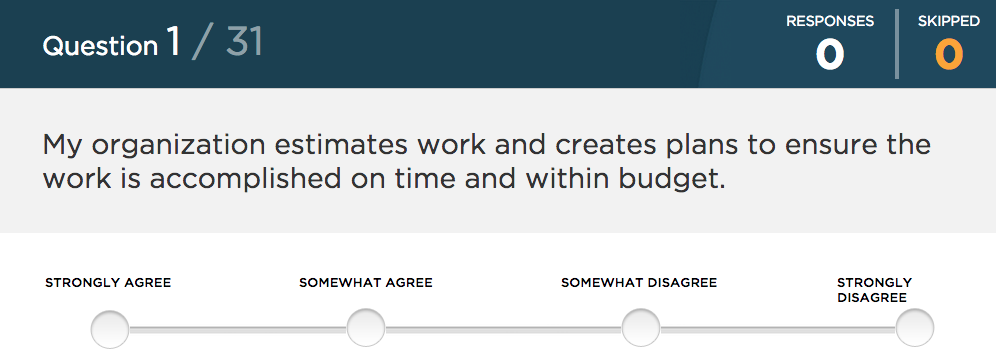
\includegraphics[width=0.75\textwidth]{cmmi_question}
		\caption{Assessment item question}
		\label{fig:cmmi_question}
	\end{center}
\end{figure}

The scale included in the assessment item also includes a descriptive information about the organization performance at both ends of the scale, visible on the example given below.

\begin{figure}[h]
	\begin{center}
		\leavevmode
		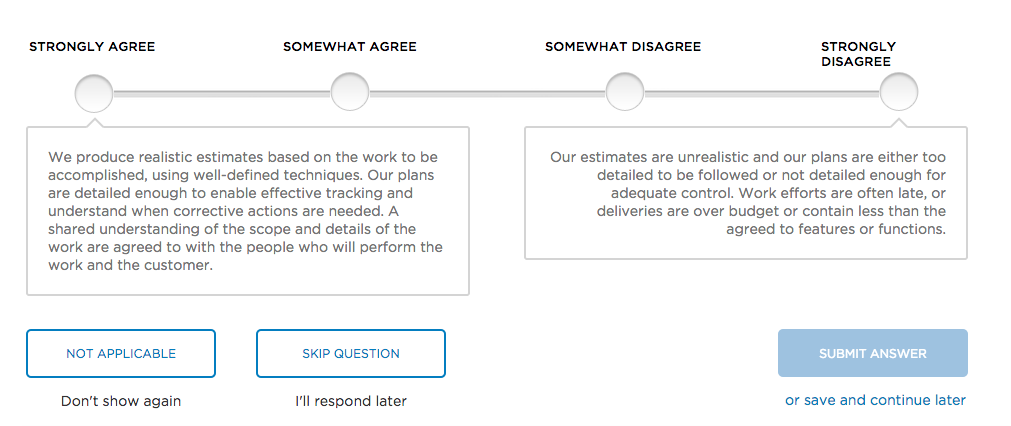
\includegraphics[width=0.86\textwidth]{respostascmmiassessment}
		\caption{Assessment item scale}
		\label{fig:assesment_answer}
	\end{center}
\end{figure}

These descriptions are given to the user with the intention of helping the most accurate positioning of the organization on the scale.

Organization term is defined by the user for purposes of  self-assessment. The evaluated scope is also by the user and can be the company, organizational unit, division, directorate, department or work group.

Its possible to skip a question in the list of items and comeback later to answer and there is an option named Not Applicable to exclude the question from the results, and this answer only should be choose if:
\begin{itemize}
	\item Actual question is related to an area outside of the organization scope.
	\item Its valid for the organization's but the  performance of the activities is not known.
	\item The user that is performing the assessment don't have sufficient expertise in the subject to understand the intent of the question.
\end{itemize}

The answers are editable before the submission of the assessment in a screen for a final review, is possible to save the current state and progress at any time and resume it later. Is only possible to submit and get an assessment if all questions are answered.

After answering all questions provided as requirement and those survey submitted will be show a high level snapshot of the organization  current capability states and will be included in each item some suggestions for developing the next steps.

\newpage

\begin{figure}[h]
	\begin{center}
		\leavevmode
		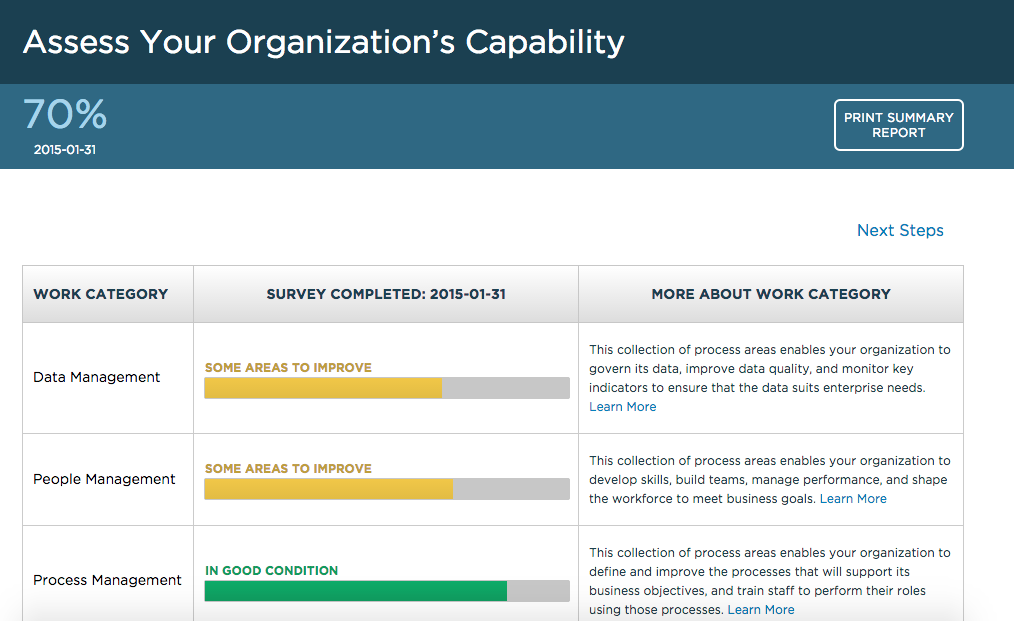
\includegraphics[width=0.96\textwidth]{resultcmmiassessment}
		\caption{Example of a result an assessment}
		\label{fig:assesment_result}
	\end{center}
\end{figure}


\section{PSP/TSP assessment checklists and tools}

PSP\citep{humphrey2005psp} is a process framework with the objective of guide developers to define their own processes, track and plan their work and manage the quality of the produced products.


\subsection{PSPchecker}

PSPChecker\citep{Pinto2010} is a tool that has the main objective of helping teachers to make decisions faster and help students to be able to achieve better results and understand PSP.

The PSPChecker was only made and planned for teachers as a support for evaluation and feedback it's suitable for students too depending on the type of teaching, that way they can improve their work. A short period of time is required to uses this tool and is currently only as a desktop application.


This desktop application has as main functionalities:
\begin{itemize}
	\item Automatic verification of checklists
	\subitem Each checklist item has different types of verification and as output if an item in the checklist is completely satisfied, it is shown the line in green otherwise red line is shown or given a special message on the screen.
	\item Custom processes
	\subitem The user when start the program can choose which items of the PSP process want to associate with this evaluation.
	\item Remote data importation
	\item Illustrative charts
	\subitem Charts that facilitate the perception of whats is wrong and well done to understand which points can be improved.
	\item Automation of support messages (use of knowledge acquired by specialists)
	\subitem Messages provided by specialist to understand the errors in a more complex level.
	\item Information Import/Export
	\begin{figure}[h]
		\begin{center}
			\leavevmode
			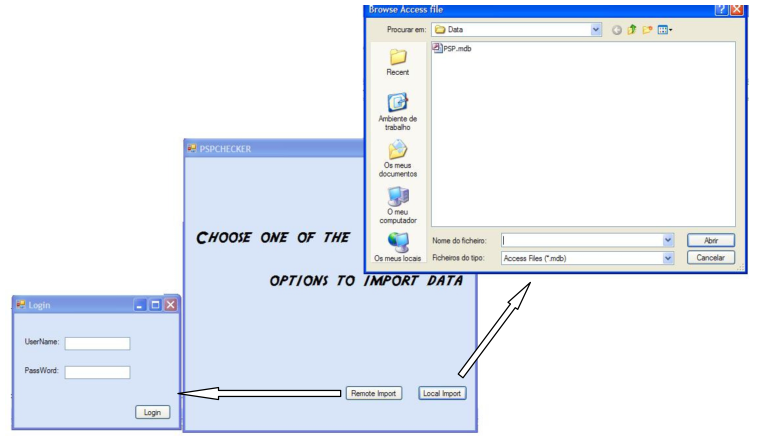
\includegraphics[width=0.63\textwidth]{PSPdataimport}
			\caption{Example of a data import for PSPChecker}
			\label{fig:PSPdataimport}
		\end{center}
	\end{figure}
	\item Modularity and scalability
\end{itemize}

\begin{figure}[h]
	\begin{center}
		\leavevmode
		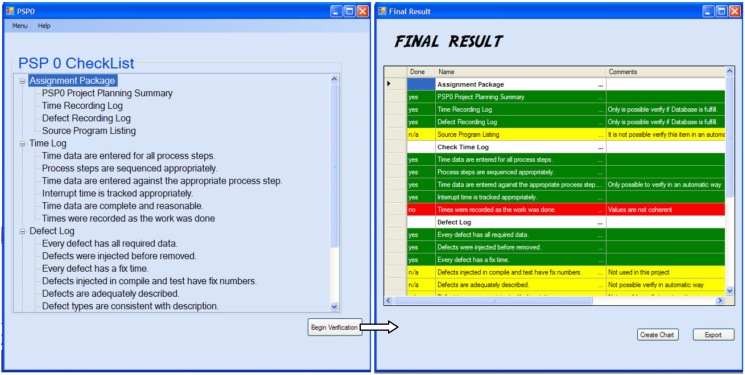
\includegraphics[width=0.8\textwidth]{PSPresult}
		\caption{Final results of PSPChecker}
		\label{fig:PSPdataimport}
	\end{center}
\end{figure}

In the Figure \ref{fig:PSPdataimport} is represented two of the last screens of PSPChecker. Is shown on the left side the checklist imported or chosen and on the right side the final screen, where we can generate charts and export the data.

\section{Appraisal Assistant}

The Software Quality Institute of the Griffith University\citep{SoftwareQuality2015} developed Appraisal Assistant. The Appraisal Assistant\citep{Appraisal2015} is a software application that supports the appraisal or assessment of process capability or organization maturity.

This tool follows consistent approaches with the requirements of ISO/IEC 15504(Information technology: Process assessment, and the Assessment Requirements for CMMI)\citep{ISOIEC} and it's distinguished from other tools by taking an evidence-driven approach to the record of evidences generated in an assessment.

SQI personnels have performed SCAMPI A and B appraisals and SPICE assessments with the help of Appraisal Assistant and have been using since the first beta release. The Beta release was used to examine relationships between ISO 15504-2 and SCAMPI appraisals

\begin{figure}[h]
	\begin{center}
		\leavevmode
		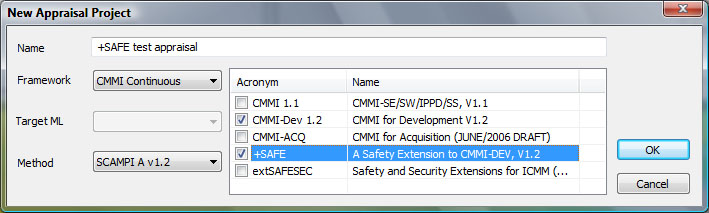
\includegraphics[width=0.8\textwidth]{newprojectsappraisal}
		\caption{Appraisal Assistant New Project Screen}
		\label{fig:newprojectsappraisal}
	\end{center}
\end{figure}

The Appraisal Assistant has many functionalities and can provide:
\begin{itemize}
	\item Support for multiple process models as: ISO/IEC 15504-5, ISO/IEC 15504-6 (FDIS), Automotive SPICE, CMMI®-DEV v.1.2, +SAFE, and CMMI® SE/SW/IPPD/SS V 1.1.
	\item User defined appraisal models.
	\item Multiple methods for performing appraisal / assessment.
	\item User defined assessment methods.
	\begin{figure}[h]
		\begin{center}
			\leavevmode
			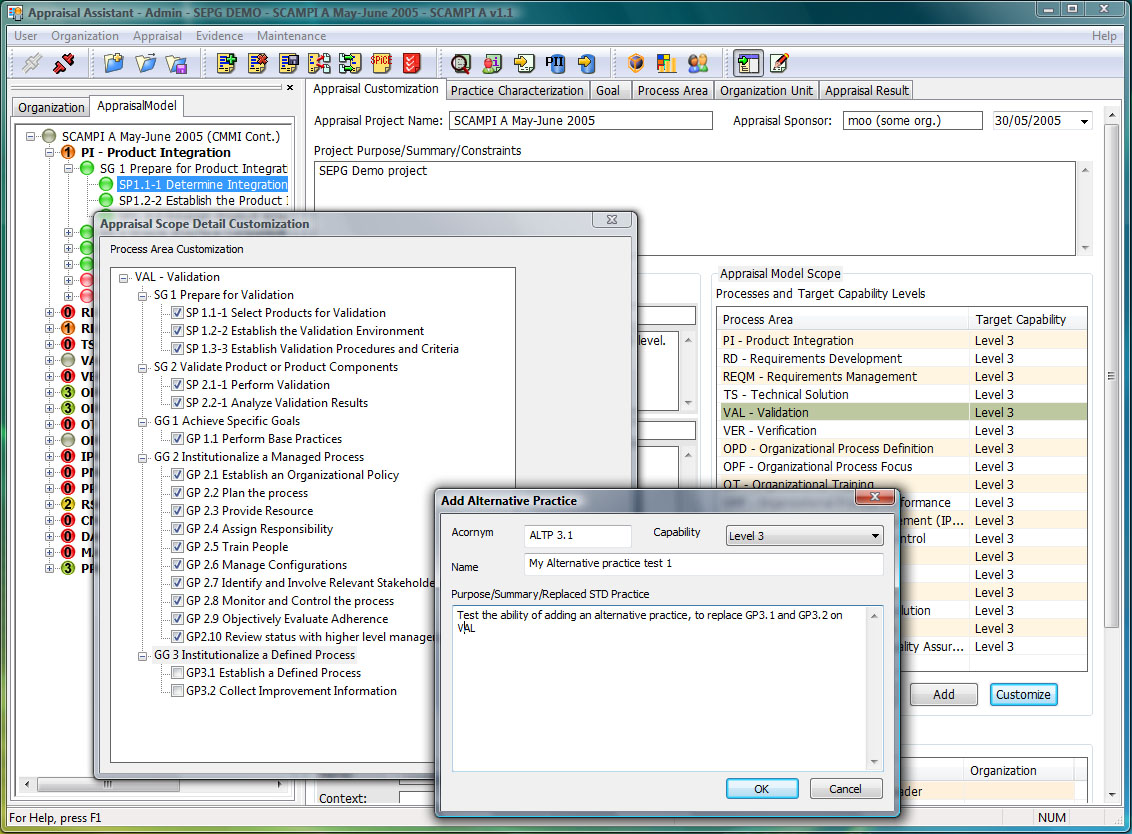
\includegraphics[width=0.6\textwidth]{cmmi_plan}
			\caption{Appraisal Scope Customization}
			\label{fig:cmmi_plan}
		\end{center}
	\end{figure}
	\item Conversion of results between frameworks
	\item Easy to split and consolidate evidence capture activities.
	\item Generate automatically reports as Appraisal Disclosure Statement, PIID, Assessment Record, Appraisal / Assessment Findings, Strength / Weakness summaries, Rating Profiles, and workload summaries.
	\item Model coverage and automatic reporting by collected evidence.
\end{itemize}


\begin{figure}[h]
	\begin{center}
		\leavevmode
		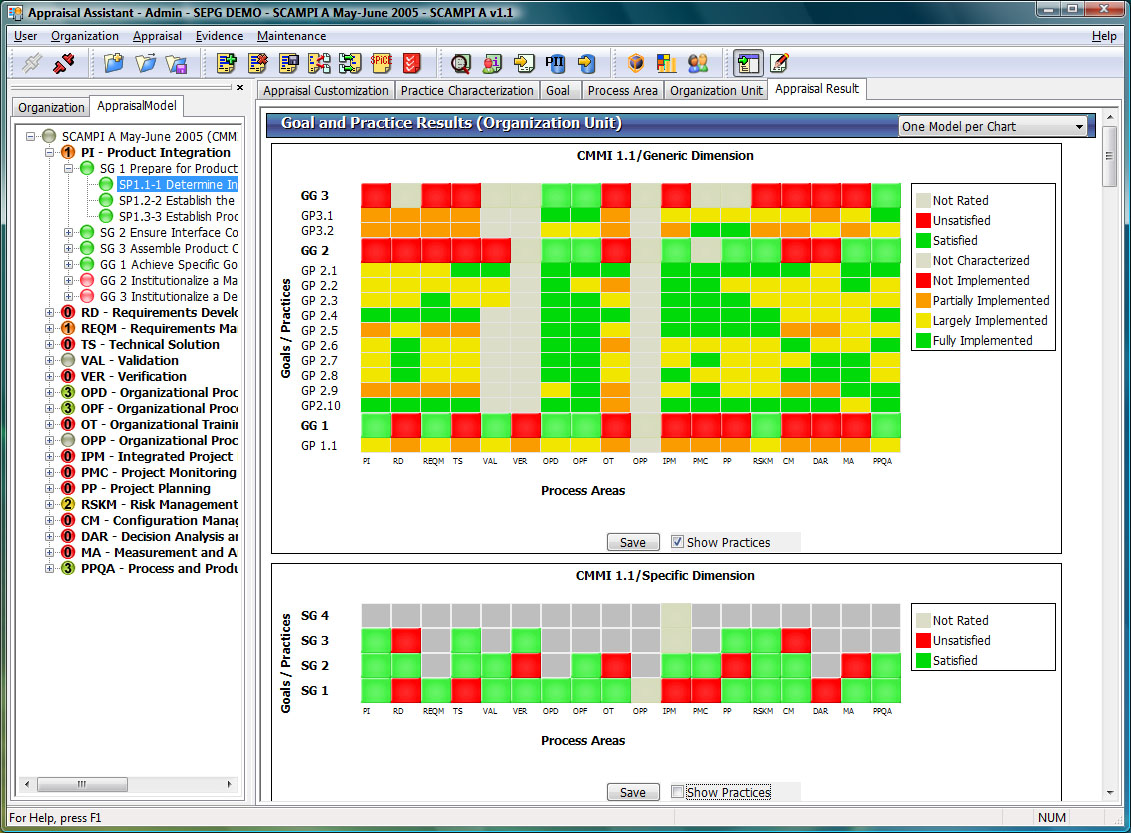
\includegraphics[width=0.6\textwidth]{cmmi_result}
		\caption{Appraisal Assistant Results}
		\label{fig:cmmi_result}
	\end{center}
\end{figure}

The Figure \ref{fig:cmmi_result} shows us an example of an appraisal result and output of the program after labeling all the process areas.
\newpage


\section{ITMark Appraisal tool}

ITmark is a certification scheme designed specifically for SMEs that combines various improvement models streamlined into only one scheme.

Is a certification developed by leading appraisal providers across technical and business related disciplines gathered in an International Consortium of Centers of Excellence dedicated to support Software Intensive Organizations throughout the world.

This certification assesses and certifies the processes in small organization in three different areas:
\begin{itemize}
	\item Business Management
	\item Software, Systems and Services Engineering
	\item Security Management
\end{itemize}

It provides a group of analysis tools that help a company enhance its business, information security management and software development processes. A company can have additional recognition for their level of capability through ITMark certification.

ITMark will provide organizations:
\begin{itemize}
	\item Process improvement of product development and services
	\item Improvement of other critical processes of the organization: business and security
	\item Low cost and quick implementation of the improvements
	\item Philosophy of quality
	\item Internationally recognized
\end{itemize}

The ITMark Appraisal tool fully support supports this process.
